\documentclass[onecolumn]{article}
\usepackage{graphicx}
\usepackage{float}
\usepackage{amsmath}
\restylefloat{figure}
\begin{document}

\title{Sum of variates}

\author{Arjen Markus}

\maketitle

\section*{Introduction}
During my PhD research I struggled to estimate the release of certain
substances (nanoparticles, actually) by people using personal care products
containing these substances. The main problem was the almost complete lack of data.
Information on how much of these products are used by different groups of people
was one thing, but finding out how much of the substances in question were present
was quite another. At some point I was able to "guestimate" the annual release
and so I used these numbers, however rough and inaccurate they may be. But it
did make me think, especially after reading this article by Ferson et al.\ \cite{UnknownDistributions}.

The task I had set myself does not have a definite answer, of course. Some estimation
is the best you can achieve, but quite often, if we encounter something along these
lines, we will assume a \emph{uniform distribution} as the ideal distribution for things
we know very little about: a minimum and a maximum suffice. The authors of the article
argue that even a uniform distribution inherently entails much more.

Let us simplfy the estimation problem: we have $N$ people that use an unknown amount $q$
of the substance of interest per year. We only know that the amount lies between some
minimum (0 grams, say) and a maximum. So, a uniform distribution might be a useful
approximation of the actual usage. The total amount these people use is therefore somewhere
between $0$ and $N\cdot q$.

However, we realise that the group of $N$ people is not homogeneous: we can distinguish
men and women, for a start, and it is unlikely that they all use the same personal care
products with the same amount of this substance. So, it would be wise to distinguish these
two groups. To keep it simple: let us say we have $N/2$ men and $N/2$ women and, again
for the sake of simplicity, they use products that contain this substance to roughly the
same amount -- $q$. Then the total release of the substance by men will be somewhere
between $0$ and $N \cdot q/2$ and the same for the release by women. Both contributions
are uniformly distributed, so we get a total release that is actually the sum
of two uniformly distributed variables. The distribution of this total is no longer
uniform, but follows a triangular shape \cite{UniformSumDistribution}.

We can go even further: it is unlikely that "younger" people will use the same
personal care products as "older" people. So, instead of two groups, we are actually
dealing with four groups! For simplicity, again, the four groups consist of the
same number of people and the range of the amount of substance that is used in the
personal care products is the same for the four.

\begin{figure}
\begin{center}
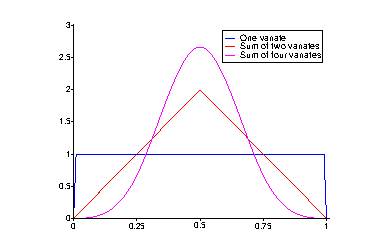
\includegraphics[width=.7\textwidth]{uniform_distros.pdf}
\caption{Shapes of the distributions for sums of one, two and four variates.}
\label{distrib}
\end{center}
\end{figure}

The resulting distribution and the distributions for the other two cases are
shown in Figure \ref{distrib}. As can be seen, the distributions are getting
narrower, the more groups we introduce, and therefore the uncertainty (variance) is
reduced. \emph{Without us getting more concrete information.}

\begin{figure}
\begin{center}
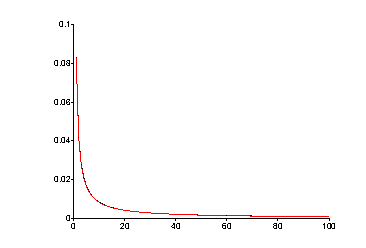
\includegraphics[width=.7\textwidth]{uniform_variance.pdf}
\caption{Variance as a function of the number of groups.}
\label{variance}
\end{center}
\end{figure}

If you were to continue this line of reasoning with ever more groups, in the
end the uncertainty would be reduced to as small a value as you want. This is
illustrated in Figure \ref{variance}. The variance for the sum of $M$ groups was
estimated by examining 100,000 sets of $M$ uniformly distributed random numbers.
The curve that resulted is actually very close to the function $V(M)$:
\begin{eqnarray}
\nonumber V(M) = \frac{1}{12M}
\end{eqnarray}

\noindent where the factor $1/12$ comes from the variance of a single uniformly
distributed number. \emph{Note:} I have not tried to determine this relation theoretically,
it was merely a hunch.

It does seem odd, that you can make a wide distribution, like the uniform
distribution, much narrower, i.e.\ having a much smaller variance, by simply
splitting up the set of individual contributions into separate groups.

\bibliography{sum-of-variates}
\bibliographystyle{unsrt}
\end{document}
